
%% bare_jrnl.tex
%% V1.4b
%% 2015/08/26
%% by Michael Shell
%% see http://www.michaelshell.org/
%% for current contact information.
%%
%% This is a skeleton file demonstrating the use of IEEEtran.cls
%% (requires IEEEtran.cls version 1.8b or later) with an IEEE
%% journal paper.
%%
%% Support sites:
%% http://www.michaelshell.org/tex/ieeetran/
%% http://www.ctan.org/pkg/ieeetran
%% and
%% http://www.ieee.org/

%%*************************************************************************
%% Legal Notice:
%% This code is offered as-is without any warranty either expressed or
%% implied; without even the implied warranty of MERCHANTABILITY or
%% FITNESS FOR A PARTICULAR PURPOSE! 
%% User assumes all risk.
%% In no event shall the IEEE or any contributor to this code be liable for
%% any damages or losses, including, but not limited to, incidental,
%% consequential, or any other damages, resulting from the use or misuse
%% of any information contained here.
%%
%% All comments are the opinions of their respective authors and are not
%% necessarily endorsed by the IEEE.
%%
%% This work is distributed under the LaTeX Project Public License (LPPL)
%% ( http://www.latex-project.org/ ) version 1.3, and may be freely used,
%% distributed and modified. A copy of the LPPL, version 1.3, is included
%% in the base LaTeX documentation of all distributions of LaTeX released
%% 2003/12/01 or later.
%% Retain all contribution notices and credits.
%% ** Modified files should be clearly indicated as such, including  **
%% ** renaming them and changing author support contact information. **
%%*************************************************************************

% *** Authors should verify (and, if needed, correct) their LaTeX system  ***
% *** with the testflow diagnostic prior to trusting their LaTeX platform ***
% *** with production work. The IEEE's font choices and paper sizes can   ***
% *** trigger bugs that do not appear when using other class files.       ***                          ***
% The testflow support page is at:
% http://www.michaelshell.org/tex/testflow/

\documentclass[journal]{IEEEtran}
%
% If IEEEtran.cls has not been installed into the LaTeX system files,
% manually specify the path to it like:
% \documentclass[journal]{../sty/IEEEtran}

% Some very useful LaTeX packages include:
% (uncomment the ones you want to load)


% *** MISC UTILITY PACKAGES ***
%
%\usepackage{ifpdf}
% Heiko Oberdiek's ifpdf.sty is very useful if you need conditional
% compilation based on whether the output is pdf or dvi.
% usage:
% \ifpdf
%   % pdf code
% \else
%   % dvi code
% \fi
% The latest version of ifpdf.sty can be obtained from:
% http://www.ctan.org/pkg/ifpdf
% Also, note that IEEEtran.cls V1.7 and later provides a builtin
% \ifCLASSINFOpdf conditional that works the same way.
% When switching from latex to pdflatex and vice-versa, the compiler may
% have to be run twice to clear warning/error messages.

% *** CITATION PACKAGES ***
%
\usepackage{cite}
% cite.sty was written by Donald Arseneau
% V1.6 and later of IEEEtran pre-defines the format of the cite.sty package
% \cite{} output to follow that of the IEEE. Loading the cite package will
% result in citation numbers being automatically sorted and properly
% "compressed/ranged". e.g., [1], [9], [2], [7], [5], [6] without using
% cite.sty will become [1], [2], [5]--[7], [9] using cite.sty. cite.sty's
% \cite will automatically add leading space, if needed. Use cite.sty's
% noadjust option (cite.sty V3.8 and later) if you want to turn this off
% such as if a citation ever needs to be enclosed in parenthesis.
% cite.sty is already installed on most LaTeX systems. Be sure and use
% version 5.0 (2009-03-20) and later if using hyperref.sty.
% The latest version can be obtained at:
% http://www.ctan.org/pkg/cite
% The documentation is contained in the cite.sty file itself.

% *** GRAPHICS RELATED PACKAGES ***
%
\ifCLASSINFOpdf
  \usepackage[pdftex]{graphicx}
  % declare the path(s) where your graphic files are
  \graphicspath{{../pdf/}{../jpeg/}}
  % and their extensions so you won't have to specify these with
  % every instance of \includegraphics
  \DeclareGraphicsExtensions{.pdf,.jpeg,.png}
\else
  % or other class option (dvipsone, dvipdf, if not using dvips). graphicx
  % will default to the driver specified in the system graphics.cfg if no
  % driver is specified.
  \usepackage[dvips]{graphicx}
  % declare the path(s) where your graphic files are
  \graphicspath{{../eps/}}
  % and their extensions so you won't have to specify these with
  % every instance of \includegraphics
  \DeclareGraphicsExtensions{.eps}
\fi%

%% it is recomended to use ``\autoref{sec:bla}'' instead of ``Fig.~Fig.~\ref{sec:bla}''
\graphicspath{{figures/}{pictures/}{images/}{./}} % where to search for the images
% graphicx was written by David Carlisle and Sebastian Rahtz. It is
% required if you want graphics, photos, etc. graphicx.sty is already
% installed on most LaTeX systems. The latest version and documentation
% can be obtained at: 
% http://www.ctan.org/pkg/graphicx
% Another good source of documentation is "Using Imported Graphics in
% LaTeX2e" by Keith Reckdahl which can be found at:
% http://www.ctan.org/pkg/epslatex
%
% latex, and pdflatex in dvi mode, support graphics in encapsulated
% postscript (.eps) format. pdflatex in pdf mode supports graphics
% in .pdf, .jpeg, .png and .mps (metapost) formats. Users should ensure
% that all non-photo figures use a vector format (.eps, .pdf, .mps) and
% not a bitmapped formats (.jpeg, .png). The IEEE frowns on bitmapped formats
% which can result in "jaggedy"/blurry rendering of lines and letters as
% well as large increases in file sizes.
%
% You can find documentation about the pdfTeX application at:
% http://www.tug.org/applications/pdftex

% *** MATH PACKAGES ***
%
%\usepackage{amsmath}
% A popular package from the American Mathematical Society that provides
% many useful and powerful commands for dealing with mathematics.
%
% Note that the amsmath package sets \interdisplaylinepenalty to 10000
% thus preventing page breaks from occurring within multiline equations. Use:
%\interdisplaylinepenalty=2500
% after loading amsmath to restore such page breaks as IEEEtran.cls normally
% does. amsmath.sty is already installed on most LaTeX systems. The latest
% version and documentation can be obtained at:
% http://www.ctan.org/pkg/amsmath

% *** SPECIALIZED LIST PACKAGES ***
%
%\usepackage{algorithmic}
% algorithmic.sty was written by Peter Williams and Rogerio Brito.
% This package provides an algorithmic environment fo describing algorithms.
% You can use the algorithmic environment in-text or within a figure
% environment to provide for a floating algorithm. Do NOT use the algorithm
% floating environment provided by algorithm.sty (by the same authors) or
% algorithm2e.sty (by Christophe Fiorio) as the IEEE does not use dedicated
% algorithm float types and packages that provide these will not provide
% correct IEEE style captions. The latest version and documentation of
% algorithmic.sty can be obtained at:
% http://www.ctan.org/pkg/algorithms
% Also of interest may be the (relatively newer and more customizable)
% algorithmicx.sty package by Szasz Janos:
% http://www.ctan.org/pkg/algorithmicx

% *** ALIGNMENT PACKAGES ***
%
%\usepackage{array}
% Frank Mittelbach's and David Carlisle's array.sty patches and improves
% the standard LaTeX2e array and tabular environments to provide better
% appearance and additional user controls. As the default LaTeX2e table
% generation code is lacking to the point of almost being broken with
% respect to the quality of the end results, all users are strongly
% advised to use an enhanced (at the very least that provided by array.sty)
% set of table tools. array.sty is already installed on most systems. The
% latest version and documentation can be obtained at:
% http://www.ctan.org/pkg/array

% IEEEtran contains the IEEEeqnarray family of commands that can be used to
% generate multiline equations as well as matrices, tables, etc., of high
% quality.

% *** SUBFIGURE PACKAGES ***
%\ifCLASSOPTIONcompsoc
%  \usepackage[caption=false,font=normalsize,labelfont=sf,textfont=sf]{subfig}
%\else
%  \usepackage[caption=false,font=footnotesize]{subfig}
%\fi
% subfig.sty, written by Steven Douglas Cochran, is the modern replacement
% for subfigure.sty, the latter of which is no longer maintained and is
% incompatible with some LaTeX packages including fixltx2e. However,
% subfig.sty requires and automatically loads Axel Sommerfeldt's caption.sty
% which will override IEEEtran.cls' handling of captions and this will result
% in non-IEEE style figure/table captions. To prevent this problem, be sure
% and invoke subfig.sty's "caption=false" package option (available since
% subfig.sty version 1.3, 2005/06/28) as this is will preserve IEEEtran.cls
% handling of captions.
% Note that the Computer Society format requires a larger sans serif font
% than the serif footnote size font used in traditional IEEE formatting
% and thus the need to invoke different subfig.sty package options depending
% on whether compsoc mode has been enabled.
%
% The latest version and documentation of subfig.sty can be obtained at:
% http://www.ctan.org/pkg/subfig

% *** FLOAT PACKAGES ***
%
%\usepackage{fixltx2e}
% fixltx2e, the successor to the earlier fix2col.sty, was written by
% Frank Mittelbach and David Carlisle. This package corrects a few problems
% in the LaTeX2e kernel, the most notable of which is that in current
% LaTeX2e releases, the ordering of single and double column floats is not
% guaranteed to be preserved. Thus, an unpatched LaTeX2e can allow a
% single column figure to be placed prior to an earlier double column
% figure.
% Be aware that LaTeX2e kernels dated 2015 and later have fixltx2e.sty's
% corrections already built into the system in which case a warning will
% be issued if an attempt is made to load fixltx2e.sty as it is no longer
% needed.
% The latest version and documentation can be found at:
% http://www.ctan.org/pkg/fixltx2e

%\usepackage{stfloats}
% stfloats.sty was written by Sigitas Tolusis. This package gives LaTeX2e
% the ability to do double column floats at the bottom of the page as well
% as the top. (e.g., "\begin{figure*}[!b]" is not normally possible in
% LaTeX2e). It also provides a command:
%\fnbelowfloat
% to enable the placement of footnotes below bottom floats (the standard
% LaTeX2e kernel puts them above bottom floats). This is an invasive package
% which rewrites many portions of the LaTeX2e float routines. It may not work
% with other packages that modify the LaTeX2e float routines. The latest
% version and documentation can be obtained at:
% http://www.ctan.org/pkg/stfloats
% Do not use the stfloats baselinefloat ability as the IEEE does not allow
% \baselineskip to stretch. Authors submitting work to the IEEE should note
% that the IEEE rarely uses double column equations and that authors should try
% to avoid such use. Do not be tempted to use the cuted.sty or midfloat.sty
% packages (also by Sigitas Tolusis) as the IEEE does not format its papers in
% such ways.
% Do not attempt to use stfloats with fixltx2e as they are incompatible.
% Instead, use Morten Hogholm'a dblfloatfix which combines the features
% of both fixltx2e and stfloats:
%
% \usepackage{dblfloatfix}
% The latest version can be found at:
% http://www.ctan.org/pkg/dblfloatfix

%\ifCLASSOPTIONcaptionsoff
%  \usepackage[nomarkers]{endfloat}
% \let\MYoriglatexcaption\caption
% \renewcommand{\caption}[2][\relax]{\MYoriglatexcaption[#2]{#2}}
%\fi
% endfloat.sty was written by James Darrell McCauley, Jeff Goldberg and 
% Axel Sommerfeldt. This package may be useful when used in conjunction with 
% IEEEtran.cls'  captionsoff option. Some IEEE journals/societies require that
% submissions have lists of figures/tables at the end of the paper and that
% figures/tables without any captions are placed on a page by themselves at
% the end of the document. If needed, the draftcls IEEEtran class option or
% \CLASSINPUTbaselinestretch interface can be used to increase the line
% spacing as well. Be sure and use the nomarkers option of endfloat to
% prevent endfloat from "marking" where the figures would have been placed
% in the text. The two hack lines of code above are a slight modification of
% that suggested by in the endfloat docs (section 8.4.1) to ensure that
% the full captions always appear in the list of figures/tables - even if
% the user used the short optional argument of \caption[]{}.
% IEEE papers do not typically make use of \caption[]'s optional argument,
% so this should not be an issue. A similar trick can be used to disable
% captions of packages such as subfig.sty that lack options to turn off
% the subcaptions:
% For subfig.sty:
% \let\MYorigsubfloat\subfloat
% \renewcommand{\subfloat}[2][\relax]{\MYorigsubfloat[]{#2}}
% However, the above trick will not work if both optional arguments of
% the \subfloat command are used. Furthermore, there needs to be a
% description of each subfigure *somewhere* and endfloat does not add
% subfigure captions to its list of figures. Thus, the best approach is to
% avoid the use of subfigure captions (many IEEE journals avoid them anyway)
% and instead reference/explain all the subfigures within the main caption.
% The latest version of endfloat.sty and its documentation can obtained at:
% http://www.ctan.org/pkg/endfloat
%
% The IEEEtran \ifCLASSOPTIONcaptionsoff conditional can also be used
% later in the document, say, to conditionally put the References on a 
% page by themselves.

% *** PDF, URL AND HYPERLINK PACKAGES ***
%
%\usepackage{url}
% url.sty was written by Donald Arseneau. It provides better support for
% handling and breaking URLs. url.sty is already installed on most LaTeX
% systems. The latest version and documentation can be obtained at:
% http://www.ctan.org/pkg/url
% Basically, \url{my_url_here}.

% *** Do not adjust lengths that control margins, column widths, etc. ***
% *** Do not use packages that alter fonts (such as pslatex).         ***
% There should be no need to do such things with IEEEtran.cls V1.6 and later.
% (Unless specifically asked to do so by the journal or conference you plan
% to submit to, of course. )

% correct bad hyphenation here
\hyphenation{op-tical net-works semi-conduc-tor}

\begin{document}
%
% paper title
% Titles are generally capitalized except for words such as a, an, and, as,
% at, but, by, for, in, nor, of, on, or, the, to and up, which are usually
% not capitalized unless they are the first or last word of the title.
% Linebreaks \\ can be used within to get better formatting as desired.
% Do not put math or special symbols in the title.
\title{Attraction and radiation range: The impact of spatial awareness on the choice of business district in Shanghai}
%
%
% author names and IEEE memberships
% note positions of commas and nonbreaking spaces ( ~ ) LaTeX will not break
% a structure at a ~ so this keeps an author's name from being broken across
% two lines.
% use \thanks{} to gain access to the first footnote area
% a separate \thanks must be used for each paragraph as LaTeX2e's \thanks
% was not built to handle multiple paragraphs
%

\author{\IEEEauthorblockN{Kelin Li\IEEEauthorrefmark{1},
Yina Li\IEEEauthorrefmark{2},
Hong Yin\IEEEauthorrefmark{3}, and
Changbo Wang\IEEEauthorrefmark{4}}
\IEEEauthorblockA{\IEEEauthorrefmark{1}School of Computer Science and Software Engineering, East China Normal University, Shanghai,China}
\IEEEauthorblockA{\IEEEauthorrefmark{2}Nankai University, Tianjin, China}
\IEEEauthorblockA{\IEEEauthorrefmark{3}School of Computer Science and Software Engineering, East China Normal University, Shanghai,China}
\IEEEauthorblockA{\IEEEauthorrefmark{4}School of Computer Science and Software Engineering, East China Normal University, Shanghai,China}% <-this % stops an unwanted space
\thanks{Manuscript received December 1, 2012; revised August 26, 2015. 
Corresponding author: M. Shell (email: http://www.michaelshell.org/contact.html).}}

% note the % following the last \IEEEmembership and also \thanks - 
% these prevent an unwanted space from occurring between the last author name
% and the end of the author line. i.e., if you had this:
% 
% \author{....lastname \thanks{...} \thanks{...} }
%                     ^------------^------------^----Do not want these spaces!
%
% a space would be appended to the last name and could cause every name on that
% line to be shifted left slightly. This is one of those "LaTeX things". For
% instance, "\textbf{A} \textbf{B}" will typeset as "A B" not "AB". To get
% "AB" then you have to do: "\textbf{A}\textbf{B}"
% \thanks is no different in this regard, so shield the last } of each \thanks
% that ends a line with a % and do not let a space in before the next \thanks.
% Spaces after \IEEEmembership other than the last one are OK (and needed) as
% you are supposed to have spaces between the names. For what it is worth,
% this is a minor point as most people would not even notice if the said evil
% space somehow managed to creep in.

% The paper headers
\markboth{Journal of \LaTeX\ Class Files,~Vol.~14, No.~8, August~2015}%
{Shell \MakeLowercase{\textit{et al.}}: Bare Demo of IEEEtran.cls for IEEE Journals}
% The only time the second header will appear is for the odd numbered pages
% after the title page when using the twoside option.
% 
% *** Note that you probably will NOT want to include the author's ***
% *** name in the headers of peer review papers.                   ***
% You can use \ifCLASSOPTIONpeerreview for conditional compilation here if
% you desire.

% If you want to put a publisher's ID mark on the page you can do it like
% this:
%\IEEEpubid{0000--0000/00\$00.00~\copyright~2015 IEEE}
% Remember, if you use this you must call \IEEEpubidadjcol in the second
% column for its text to clear the IEEEpubid mark.

% use for special paper notices
%\IEEEspecialpapernotice{(Invited Paper)}

% make the title area
\maketitle

% As a general rule, do not put math, special symbols or citations
% in the abstract or keywords.
\begin{abstract}
The measurement and evaluation of the attraction and radiation range of business districts in Shanghai is examined in this paper, the city which had experienced rapid development of public transport in recent years. Convenient public transport has changed our shopping habits, which become more irregular, and business districts have different modes of development. However, the research methods based on statistics, experience and sampling have not been able to adapt to the era of big data. Here we establish an attractiveness model focus on Shanghai's business districts by mining traffic data and apply a new method with customer-oriented to division scope of radiation range. Visual analysis is used to draw the conclusion that 1)Spatial awareness is no longer the important factor negative influence shopping, 2)the factors that affect the attractiveness already from single factor (commercial area) to mixed factors (commercial area, reputation, goods grade, etc. ), and 3)psychological expectations will make customer behavior more regular. We evaluate these studies and anticipate that this work can provide decision-making assistance to governments and retail businesses. 
\end{abstract}

% Note that keywords are not normally used for peerreview papers.
\begin{IEEEkeywords}
Business district, Visual analysis, Radiation range, Attraction model.
\end{IEEEkeywords}

% For peer review papers, you can put extra information on the cover
% page as needed:
% \ifCLASSOPTIONpeerreview
% \begin{center} \bfseries EDICS Category: 3-BBND \end{center}
% \fi
%
% For peerreview papers, this IEEEtran command inserts a page break and
% creates the second title. It will be ignored for other modes.
\IEEEpeerreviewmaketitle

\section{Introduction}
% The very first letter is a 2 line initial drop letter followed
% by the rest of the first word in caps.
% 
% form to use if the first word consists of a single letter:
% \IEEEPARstart{A}{demo} file is ....
% 
% form to use if you need the single drop letter followed by
% normal text (unknown if ever used by the IEEE):
% \IEEEPARstart{A}{}demo file is ....
% 
% Some journals put the first two words in caps:
% \IEEEPARstart{T}{his demo} file is ....
% 
% Here we have the typical use of a "T" for an initial drop letter
% and "HIS" in caps to complete the first word.
\IEEEPARstart{B}{usiness} district is a geographical concept generated by aggregation of retail stores. Business district in a broad sense is a business concept which made up of shopping centers, department stores and related infrastructure, and in a narrow sense is a geographical concept with several stores.This article explores the attraction and radiation range of business districts (broad sense) in Shanghai by analyzing and mining urban public transport data and business data.

The concept of attraction of business was proposed by Reilly in 1930s, and Huff put forward the attraction model of the business district. Until now, most of the relevant research is an extension of these studies. However, different regions have their own economic level, which result the conclusions of business district research to not be universal.Now, the rapid development of public transport makes commerce more prosperous and intensive in Shanghai, and many non-commercial functions (e.g. catering, banks, government organs, etc.) have gradually moved over from individual area to the business districts. Like densely populated cities, business districts have become the center of business activities in Shanghai.

As the business activity is people-centred, a considerable part of the research on the business districts is conducted through questionnaires and sample surveys. Many valuable and interesting conclusions have been found in the existing research, but we need to use new ideas to study the business district and business activity in the era of big data. Due to balance development in Shanghai economy and commerce, customer characteristics, market competition and other factors have little discrepancy. If we fully follow the existing conclusions, we find that it does not always satisfy our research. Therefore, this work is an exploration of business district under circumstances of big data.

Business districts in Shanghai become ``energetic organs'', comprised of entertainment, shopping and leisure, and the public transport system (PTS) connects the whole body. The objective of this paper is to measure the attractiveness of the business district in Shanghai, with an emphasis on building an attraction model, a summary measure of centre attraction for potential customers, and a new angle about commercial radiation range. The methodological approach is based on information visualization, visual analysis, statistics and evaluation for a variety of different models. On the other hand, the specifics of PTS introduce an original element to the study of attraction. In addition, the variables used in this research are atypical of the most of big cities, that the process can be repeated in similar research. Thus the results of the study can be used for broader scope, but only suitable for big cities at this stage.

\begin{figure*}[tb]
\centering
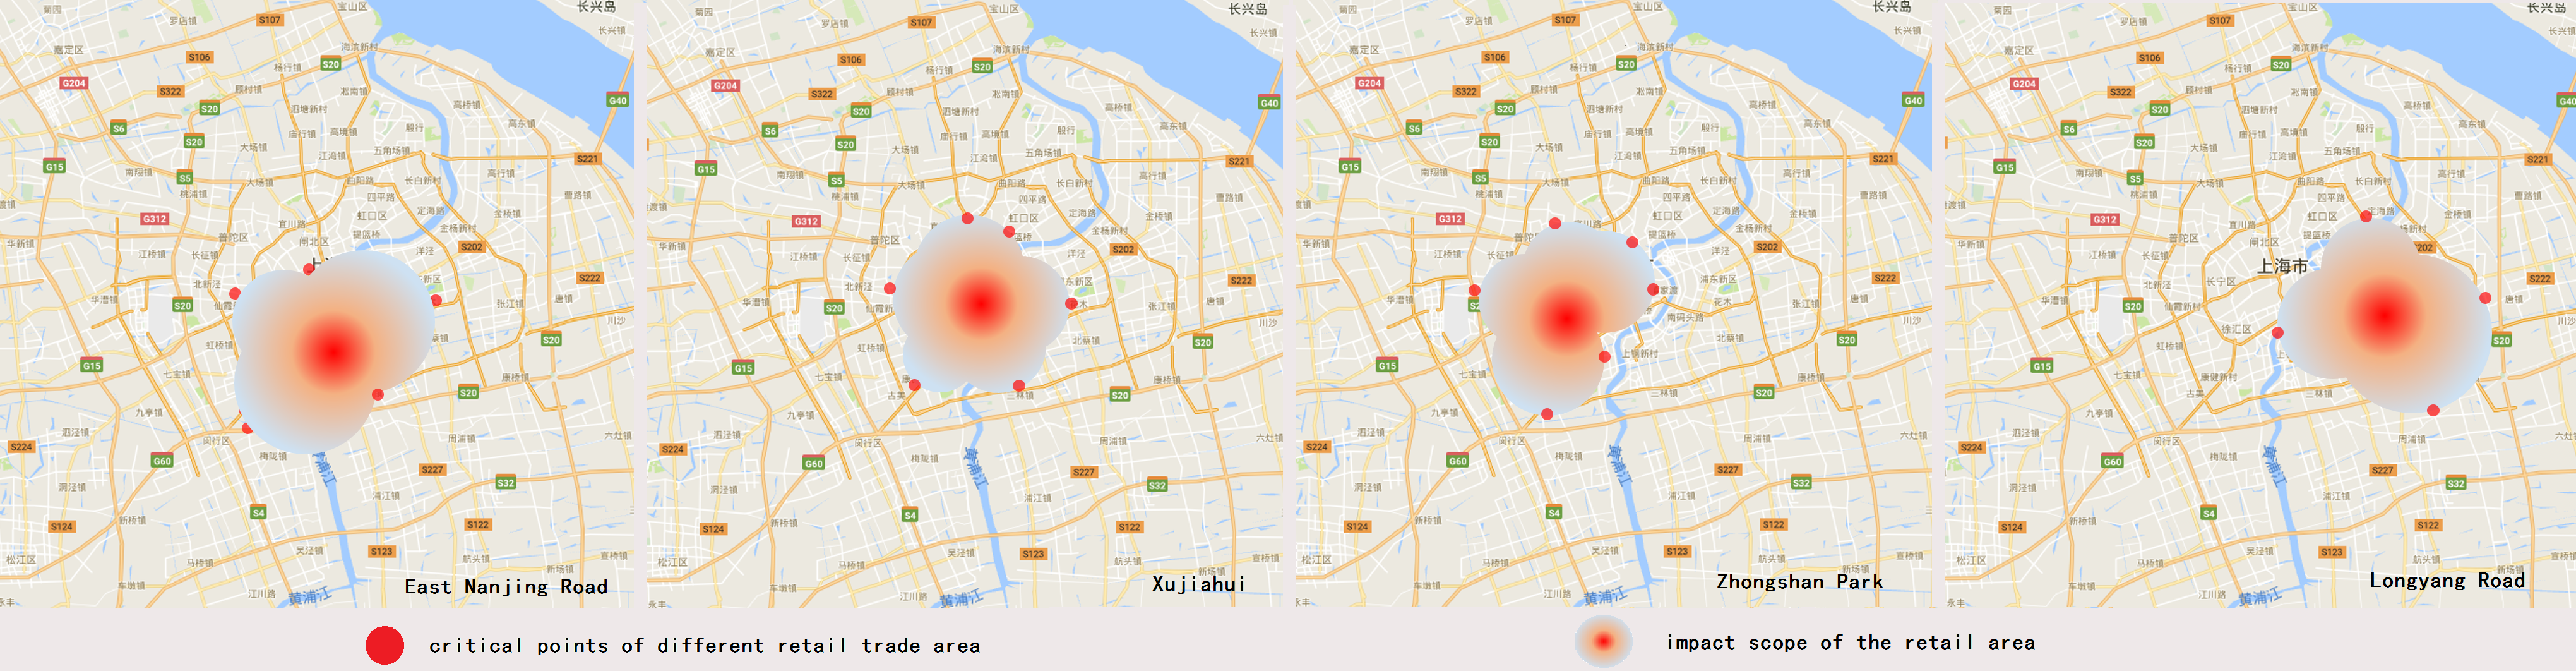
\includegraphics[width=1.9\columnwidth]{figure1.png}
\caption{Radiation range based on the resulys calculated by Reilly Rule of four different types of business districts in Shanghai.}
\label{fig:Reilly-range}
\end{figure*}

In the first place, our contribution is mainly focused on the following points:

\begin{itemize}
\item Put forward a attraction model of business district with more accurate and practical, which could calculate the degree of attractiveness from one business district to anywhere.
\item Propose a method to division and drawing the radiation range of business district, and explain its advantages by comparison with the human-centered method.
\item 
\end{itemize}

And this paper is trying to answer the following questions:
\begin{itemize}
\item Q1: Is the attractiveness of business districts can express in numerical terms? Is this the existing result and model represents the status quo of business development of Shanghai?
\item Q2: Is the attractiveness depends on a variety of factors with high degree of influence? Is there any advantage compared with previous research results? and
\item Q3: Is there a way to represent the radiation range of a business district with another view? Whether it has good application value if it exists?
\end{itemize}

This paper is divided into four sections. After the data and theoretical introduction, the crowd classification and behavior based on traffic data are discussed. The methods and attraction model used in the analysis are then designed and discussed, followed by the case studies and user surveys were conducted. In addition, the summary of the overall work and some limitations were finally proposed, and ideas for future research are discussed.

% In this paper, we extract the customer groups and establish an attraction model. And then, we evaluate the advantages of this model through visualization and draw the radiation range of customer-oriented.
% You must have at least 2 lines in the paragraph with the drop letter
% (should never be an issue)

\section{Relate Work}

\emph{Transit oriented development}. Transit oriented development (TOD) has become an increasingly popular and effective mode for analyzing a wide variety of the combination of business and traffic problems, and the era of big data brings new methods and revelations. Based on the scope and type of research, existing methods and perspectives can be roughly categorized into two types: commercial planning and traffic planning.

A research from the perspective of commercial planning describes  the positive and negative effects of the development of PTS on commerce and business district, which proposes a method for business planning in TOD mode~\cite{Allen2007Integrating,Jie2007Public}. By contrast, the research from the perspective of traffic planning is focus on the use of above-ground and underground space, in which a reasonable subway station layout will make more efficient use of space and guide passengers~\cite{Jie2007Public,Vera2014PERENCANAAN,Lu2005URBAN}. Among existing TOD mode, urban planners, economists, and project managers are using public transit as the cornerstone of their devel~\cite{N2004The}. And benefits attributable to TOD initiatives include, preservation of open space, flourished business, increased ridership and revenue~\cite{Cervero2004Transit}.

\emph{Mobility behavior}. Many works that are relevant to human mobility behaviors over public transportation system usually explore commute patterns and behavioral differences between different groups.  Wood et al.~\cite{Wood2011Visualizing} visualized flows between origins and destinations of a bicycle hire scheme. Flow maps with symbols presented overviews of bicycle traffic flow and gridded views explored docking station status over space and time. Zeng et al.~\cite{Zeng2013Visualizing} proposed the interchange circos diagram to reveal passenger distribution in a traffic network and study interchange patterns in a spatiotemporal manner.  Van der Hurk et al.~\cite{Hurk2015Deduction} presented a method for extracting the chosen routes of passengers based on smart card data from the Netherlands Rail System. Kieu et al.~\cite{Le2015Passenger} proposed a methodology for passenger segmentation from smart card data. Here, they helped transit operators understand passengers that belong to identifiable types of similar behaviors and needs.  
Furthermore, there are many works exploring the traffic flow based on mobile phone location data. Ma et al.~\cite{Ma2016Mobility} extracted trajectories across a city from mobile phone data and assisted analyst to identify typical patterns of movement by visualizing details of trajectory flows. Yang et al.~\cite{Yang2016Exploring} aimed at exploring human mobility hotspots based on mobile phone location data using kernel density estimation and clusters.

\emph{Business attraction}. Attractiveness model of the business district has been well documented in the literature of economics. Scholars have built models of attractiveness respectively for urban and suburban~\cite{Dennis2002Central,Wahlberg2016Small}, retail stores~\cite{Singla2016Investigating} and shopping malls~\cite{Dennis2002Central,Yao2016Factor}. Those models are generally based on Reilly’s rule~\cite{Reilly2006Reilly} and Huff's model~\cite{Honda1982QUANTITATIVE}. Comparing with Reilly’s rule, Huff's model can provide information on the number of customers. Therefore, one of our studies is to optimize Huff's model to calculate the attractiveness of the business district. In our work, we need to derive accurate customer flow, in order to a further assess to the maximum possible profit. However, traditional economic methods cannot meet our requirements for accuracy, so we use the machine learning and linear regression with visual analysis methods to optimize this model. To our knowledge, the problem has not been systematically using data mining and visual analysis methods. In this study, we present an optimized model of business district attractiveness. 

\emph{Spatial visualization}. Data-driven traffic visualization techniques have received noticeable attentions recently, including visualizing massive spatial data~\cite{Standart2011Geospatial}, immersive visualization VR~\cite{Berberich2009Geospatial} and the spatial visualization of time series data~\cite{Standart2011Geospatial}. Meanwhile, the visual analysis method has also developed rapidly, like the method of urban PTS~\cite{Zhang2017A} or based on the trajectory data~\cite{2016Multi}.

Geospatial data visualization is significantly changing the way we view spatial data and discover information. Our work focuses on the visual analysis of traffic data and commercial data to discover the rules hidden inside the data and then design and optimize the model of business attraction.



\section{Business District Theory and Data}

\subsection{Attraction Model}

Business district is the range of retail transactions, in this paper, it is the space range of shopping malls and department stores. The most widely used theory of business district are Reilly Rule and Huff Model, which are the earliest model. 

Detailed business information is difficult to obtained in most cases, which results a challenge about how to invest for enterprise, and Reilly Rule first provides theoretical guidance. Reilly believes that commerce also has the characteristics of mutual attraction, and then he put forward the method of the critical range of attractiveness of the business district based on the Law of Universal Gravitation. However, Reilly Rule has great limitations, and requires more stringent preconditions. A Reilly Rule calculation of business districts in Shanghai is then studied, which has complex errors due to the differences and complexity of business districts and customers behavior. The Reilly Rule we use IS as follows:
\begin{equation}
D_{ab}=d/(1+\sqrt{P_{a}/P_{b}})
\end{equation}
where $D_{ab}$ is the radiation range of business district $A$, $d$ is the distance between $A$ and $B$, and $P_{a}$, $P_{b}$ are the number of customers in this two business districts respectively.

Reilly Rule can establish the radiation range of business district, but due to it does not consider the customer uncertainty in the choice led to significant errors, and the results are shown in Fig.\ref{fig:Reilly-range}. The four business districts shown in this figure have completely different features: Xujiahui also has the position of transportation hub and financial center, Nanjing East Road has a large number of small shopping malls and attracts a large number of tourists, Zhongshan Park is an important transportation hub and Longyang Road connects the suburb and the urban area of the Pudong region. In addition, the premise of using Reilly Rule are as follow: (1) the traffic are similar; (2) the hardware properties are similar; and (3) the customer (population type and flow) are similar. In this paper, we analyze the business districts that meet these requirements.

Based on Reilly's research, Huff conducts work from the customer's point of view, quantifying the attractiveness of a business district as a probability value, which can indicate the degree that one people going to a business district. However, due to the limitations of the times, Huff only proposed a few factors for calculation, some of which are not suitable in the present society like space distance or commercial area.

Huff believes that the fundamental reason for affecting the size of the business district is that consumers engaged in shopping behavior of the psychological identity. Huff Model is as follows:
\begin{equation}
P_{ab}=\frac{\frac{S_{j}^{\mu}}{T_{ij}^{\lambda}}}{\sum_{j=1}^{n}\frac{S_{j}^{\mu}}{T_{ij}^{\lambda}}}
\end{equation}
where $P_{ij}$ is the probability where region $i$ to the business district $j$, $S_{j}$ is the attractiveness of business district $j$ and the resistance that people in region $i$ to the business distrrict $j$ is expressed by $T_{ij}$. In addition, $\mu$ and $\lambda$ are the revised values estimated on experience, $n$ is the count of business districts that have competitive relationships.

\begin{figure}[tb]
\centering
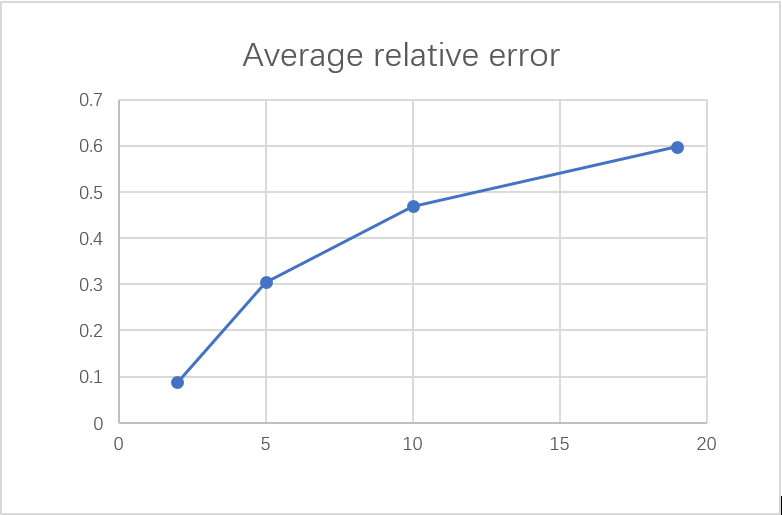
\includegraphics[width=1\columnwidth]{figure2.png}
\caption{The calculation accuracy of the number of business districts which have competitive relationships in Huff Model}
\label{fig:Huff-accuracy}
\end{figure}

We can get the value of the attractiveness of the business district by Huff Model which is similar to the actual value. However, if $n$ (the business districts that have competitive relationships in calculation) is too large, so the accuracy will be reduced with the size of the $n$ which is shown in Fig.\ref{fig:Huff-accuracy}. In addition, more factors will have impacts on the attractiveness of the business district in the current economic context, and the resistance is not only based on space distance. In this paper, we extracted a dozen factors that may have an impact on the attractiveness and resistance of the business district after interacting with a marketing manager, and a correlation study (5.1) and a attraction model (5.2) of business district are then carried out and designed.

\subsection{Input Data Set}
A large amount of data and seldom subjective factors are used in this paper, and the dataset is as follows:


\textbf{RFID public transportation card data} records passenger journeys in the Shanghai public transportation system over a typical day. This includes the metro system and the public bus network, where passengers use their personalized RFID cards to tap on card readers. The card reader system records every tap in/out action, which contains time, address, the cost and the mark of tap in/out. This dataset is about one billion and six hundred million lines in a total of four months.

\textbf{Budiness districts data} includes all the Central Business District (CBD) in Shanghai, which contains the commercial area, malls rent and etc. Commercial area is one of the most important criteria for measuring conditions, we get this data through the official website of each shopping mall or department store.

\textbf{Travel time cost} in this paper refers to the time that customer spend from a place to a CBD. The PTS in Shanghai is well-developed, so the spatial distance will cause error to the calculation results. Therefore, we introduce the concept of travel time cost instead of spatial distance as a part of the resistance factors. But it's hard to get the exact value due to each people is unique.

At first we crawled the official website data of the Shanghai Metro, and some error is found after calculating in the model. In official point, time always have to considers the worst case in PTS which causes the calculation overflowed. Therefore, we statistically analyze PTS data, and sort all the data for any two locations. As some people stay in station for some reason, we extracte the first 80 percent and calculated the average, which is the travel time cost of this two locations.

\textbf{Real attractiveness data} is a value obtained by statistical analysis and calculation. A research of people classification and shopping behavior is used to extract the customer group, a probability value is then obtained through the analysis of the classification and the traffic.

In addition, some of the data used in the calculation like the business district level, traffic station level and so on are from the government public data or network data.









\section{People Classification and Shopping Behavior}

Due to traffic jams and sparse parking spaces at the peak of the trip, most people rely on PTS, which is the artery of a city. This section focuses on exploring and analyzing human mobility behaviors from the passenger RFID card data in a PTS with a family of analytical tasks. In particular, we present an interactive visual analytics system that deals with the major challenge discovering interactively behaviors of different groups and displaying changes of the time-series traffic flow. 

The metro system plays an important role in the modern public transportation system. Salaried people rely on the metro, due to its convenience without the traffic jams. The potential movement patterns can be funded from the massive passenger RFID card data. The changes of the traffic flow with time need be displayed for a better understanding of movement trajectories. Especially, we focus on the traffic flow of office workers and analyze the residence location and the work location according to RFID card data. Our goal is that reveals features of the metro traffic flow by combining with visualization techniques. Our main analytical tasks are shown as follows: 

\textbf{T.1:} How to explore and display the changes of the traffic flow with time in different subway stations? This allows end users to understand the features of the traffic flow between different lines.

\textbf{T.2:} Measuring the traffic flow trend of between subway stations, which has large passenger flow? These subway stations reflect the main features of the subway network and movement patterns of office workers. 

The above tasks mainly focus on analyzing the traffic flow of the subway system. The solution to these tasks will empower users to select different subway lines and subway stations at a given time period. The following tasks aim at exploring characteristics and movement patterns of different groups.

\textbf{T.3:} Discovering residence location and work location of office works. The location information provides a better way to understand the movement patterns of office workers. 

\textbf{T.4:} Distinguishing different groups from the RFID card data according to its own movement patterns. For example, we can infer a person whether work overtime or not according to the frequency of going to work location.


Millions of records contain trajectories of different groups. In this paper, we focus on analyzing mobility behaviors of office works. First, trajectories of office workers need be acquired from passenger RFID card data. These office workers who take subway usually have the same journey. All journeys of an office worker have the same origin and destination during the working days. Finding office workers is modeled as follows:

\begin{equation}
W=\{w_{i}|\ { }|S_{in}|\ge4,|S_{out}|\ge4\}
\end{equation}

where $W$ is the set of all office workers in Shanghai, for each office worker $w_{i}$, there must be at least continous 4 records during working days with the same origin station and the same destination station.
Here, we define normal and abnormal office worker for further analyzing the metro flow of office workers. The normal office worker is who works for at most consecutive 5 work days. The abnormal office worker is who works at least consecutive 6 days, especially works on Saturday or Sunday or both as well. 

Office workers are more willing to take the metro, due to its convenience and low-carbon lifestyle. Furthermore, at the peak of the trip, it is difficult to take a taxi or find a parking space in Shanghai. In order to explore movement patterns of office workers, we infer the residence location and the work location of office workers based on our assumption. We suppose that office workers often choose the nearest subway station from his/her home as the origin and the nearest subway station from his/her work location as the terminal. This makes sense in line with personal experience. According to this finding, the work location and the residence location are modeled as follows:

\begin{equation}
L_{r}=\{L_{r}^i|\ 6:00< T_{in} < 9:00, Dur_{i}\ge5\}
\end{equation}
\begin{equation}
L_{w}=\{L_{w}^i|\ 17:00< T_{in} < 20:00, Dur_{i}\ge5\}
\end{equation}

where $L_{r}$ is the set of residence locations, and $L_{r}^i$ is the residence location for the ith card, if its tap-in time $T_{in}$ is between 5:00 and 10:00 a.m. and it appears for at least consecutive 5 working days with the same station. Where $L_{w}$ is the set of work locations, and $L_{w}^i$ is the work locations for the ith card, if its tap-in time $T_{in}$ is between 17:00 and 20:00 and it appears for at least consecutive 5 working days with the same station. Once the residence location and the work location are inferred, more features of different groups could be found.

Hence, the flow between two stations was displayed in flow snapshot view.  Here, the thickness of the line indicates the size of flow. As illustrated in Fig.\ref{fig:Flow-view}, the line with the color yellow, metro line 2, carries more traffic loads that other lines. Besides, a pie chart was used to display flow changes of office workers that appear at least 5 continues working days at the same residence and work location. The blue part indicated the number of going into this station; the red part indicated the number of going out this station. Then, distribution of residence location and work location was shown in Fig. 3. The region with many pie charts that have a larger number of going into this station probably contained certain residence communities. The region with pie charts that have a larger number of going out this station probably contained certain sci-tech parks. 

The research in this chapter provides support for the validation of the computational results of the attraction model.

\begin{figure}[tb]
\centering
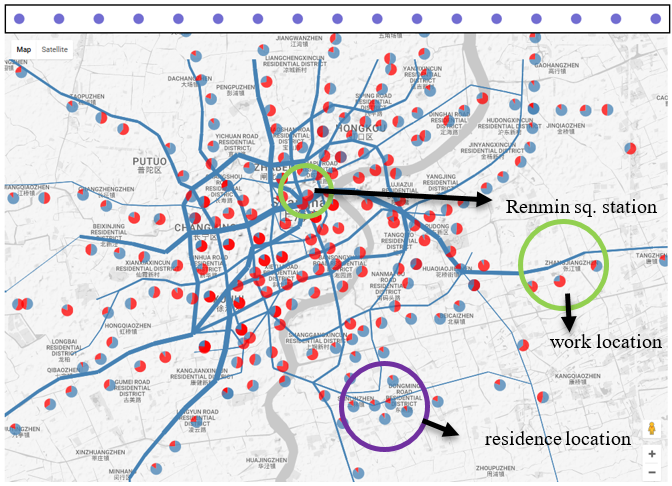
\includegraphics[width=1\columnwidth]{figure5.png}
\caption{Flow snapshot view from 6:00 pm to 6:30 pm. This view shows the metro traffic flow at a given time and pie chart indicates a number of going into and out this station.}
\label{fig:Flow-view}
\end{figure}










\section{The Attraction Model of Business District}

This section introduces the design and analysis of the attractiion model of the business district.

\subsection{Correlation and Coefficient}

The significance and correlation of the calculated variables proposed by Huff are shown in TABLE \ref{tab:correlation}. The correlation coefficient for time cost is -0.489 and for commercial area is 0.149, and both have significant correlations. After discussing with the manager, the reason we think for the small correlation coefficient is follows: The PTS in Shanghai is high developed, which result the space distance and time cost have smaller impact on people's travel; The research samples are all central business districts, which have similar commercial areas.

\begin{table}[ht]
\centering
\normalsize
\caption{The correlation of time cost and commercial area}
\begin{tabular}{|l|l|l|l|}\hline
      Variable&Probability&Time cost&Commercial area\\
      \hline
      Correlation&1.000&-0.489&0.149\\
      \hline
      Significance&.&.000&.000\\
      \hline
      Sample&5111&5111&5111\\
      \hline
\end{tabular}
\label{tab:correlation}
\end{table}

As shown in formula 2, $\mu$ and $\lambda$ are the revised values estimated on experience in Huff Model. We invite experts in related fields to help us give two values as a subjective index to make a better comparison. Meanwhile, we obtain the correlation coefficient value as an objective index through big data analysis. In addition, a constraint is proposed as $\mu+\lambda=2$ for better calculation. We got two sets of index numbers after normalization and amplification, and then we calculate the attractiveness of the business districts and the range of radiation. The two adjustment index values are like TABLE \ref{tab:adjustment-index-values}.

\begin{table}[ht]
\centering
\normalsize
\caption{Two adjustment index values}
\begin{tabular}{|l|l|l|l|l|}\hline
      &\multicolumn{2}{|c|} {subjective index}&\multicolumn{2}{|c|} {objective index}\\\hline
      Regulatory factor&$\lambda(t)$&$\mu(s)$&$\lambda(t)$&$\mu(s)$\\\hline
      Value&1.5&1.2&0.454&0.120\\\hline
      Normalized&0.556&0.444&0.791&0.209\\
      \hline
\end{tabular}
\label{tab:adjustment-index-values}
\end{table}

The results are shown by visualization techniques in Fig.\ref{fig:Five-model-compare}, where the regulatory factors were normalized and magnified.

\begin{figure*}[tb]
\centering
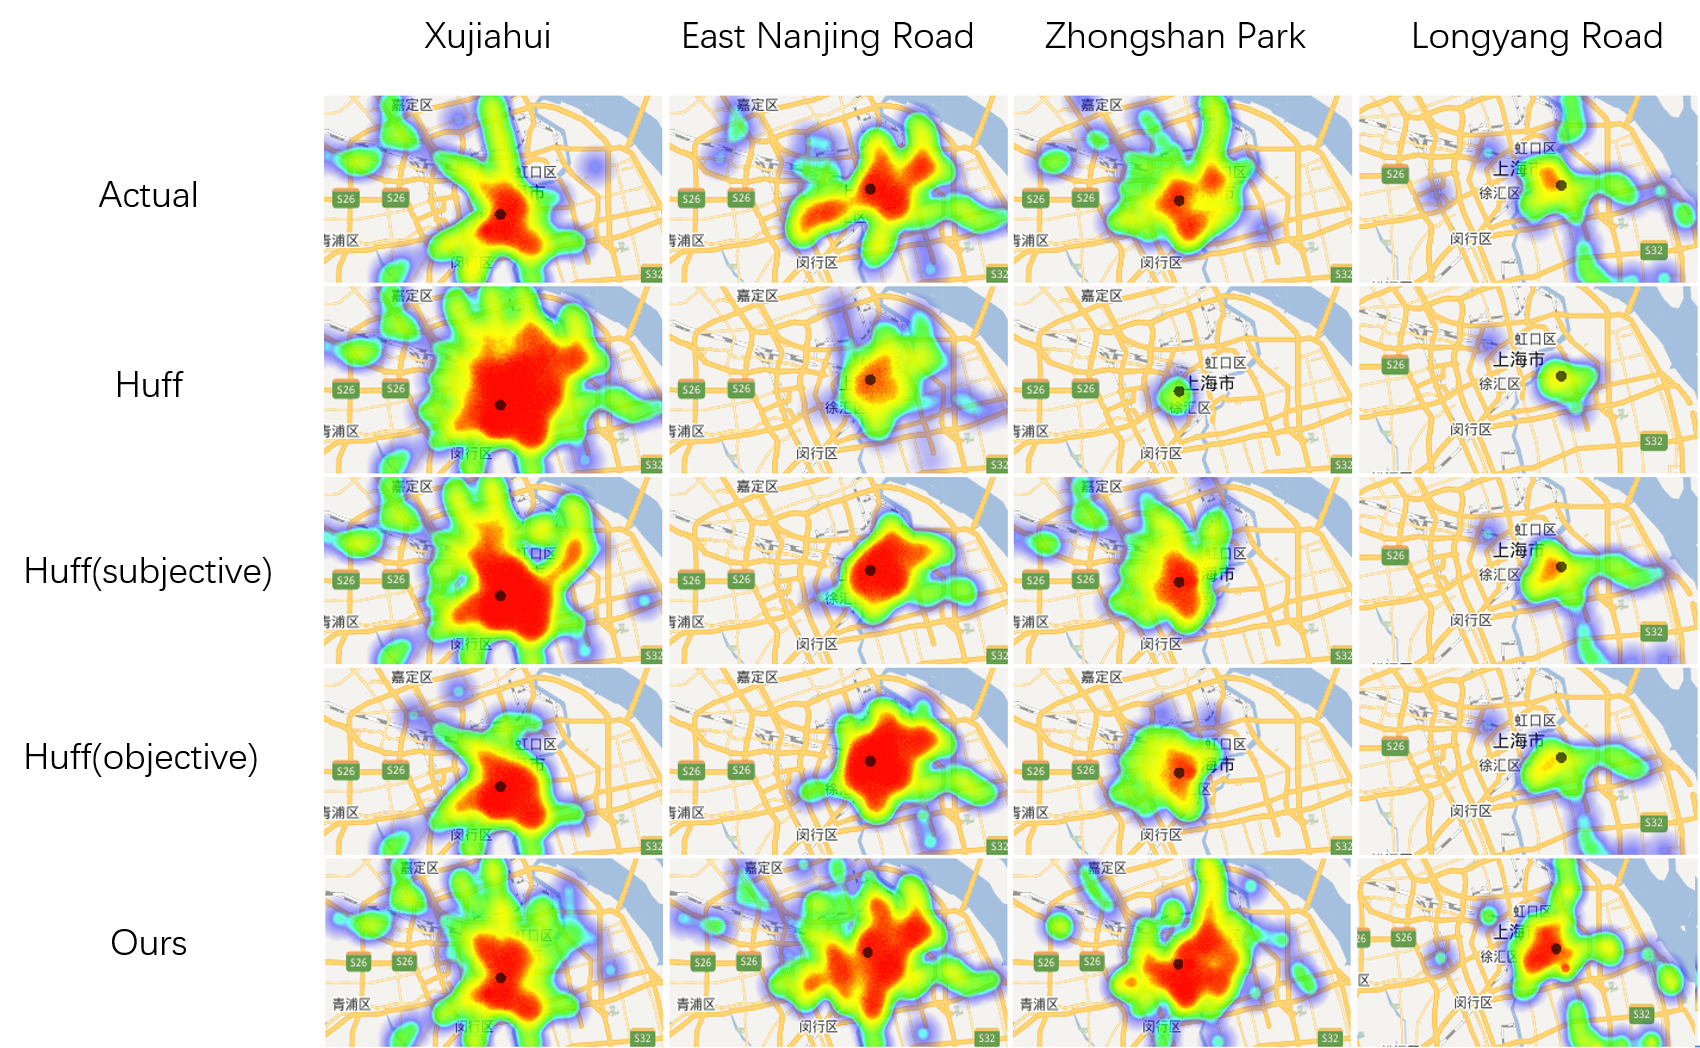
\includegraphics[width=1.8\columnwidth]{figure4.png}
\caption{A visual view of the radiation range, which are calculated from four models and raw data.}
\label{fig:Five-model-compare}
\end{figure*}

Through the visual comparison of the model calculation results, we can clearly see that the precision of the exponentially adjusted model has been significantly improved, but the two index adjustment methods do not have obvious advantages and disadvantages. We think this is due to Huff Model uses only commercial area and space distance for calculation, and in practice, the determination of charm and resistance is more complicated. In addition, in order to get more accurate results, we train the data using machine learning and get a set of values of influence factors. The possible influence factors and training results are shown in Table \ref{tab:machine-learning}.

\begin{table*}[ht]
\centering
\normalsize
\caption{The training results of machine learning}
\begin{tabular}{|l|l|l|l|l|l|}\hline
       &time cost&commercial area&commodity grade&market number&popularity\\\hline
      influence value(\%)&27.64570&36.85034&33.19354&28.09620&26.56424\\
      \hline
\end{tabular}
\label{tab:machine-learning}
\end{table*}



\subsection{Model Design}

The basis of our model design is also the law of universal gravitation. A larger commercial area and a wider variety of products can attract more consumers, which need to be considered in related research. However, in this paper, the samples are the central business districts and all are very prosperous, which result a smaller differences in attribute. Meanwhile, we can get similar conclusions: Factors such as commercial area and district level have no significant impact on attractiveness, but other ffactors, such as time cost and the count of changeovers, have a much higher impact on selection.

\begin{figure}[tb]
\centering
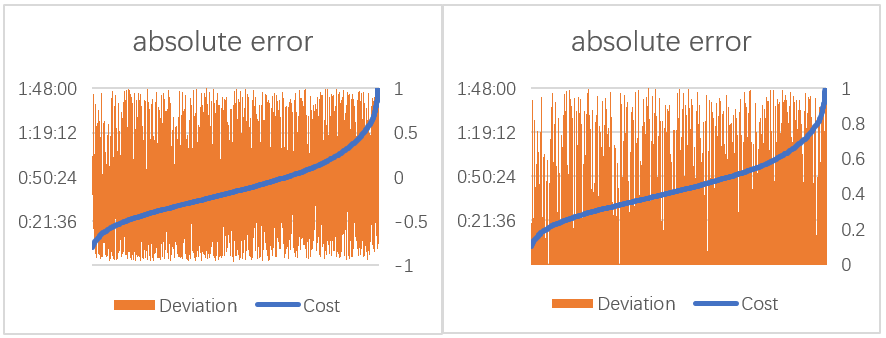
\includegraphics[width=1\columnwidth]{figure6.png}
\caption{Absolute error 1}
\label{fig:Absolute-error 1}
\end{figure}

After many validations and analyzes, we propose a model of attractiveness for Shanghai's business districts:

\begin{equation}
Attraction=Grade^{\alpha}*Mall^{\beta}*Area^{\gamma}*Reputation^{\delta} 
\end{equation}
\begin{equation}
Attractive=\frac{Attraction}{Time^{\mu}}
\end{equation}
where $\alpha$, $\beta$, $\gamma$, $\delta$ and $\mu$ are adjusted index based on data analysis and mining. We can get $Attraction$ to empress the charm, and $Attractive$ to represent the degree of attraction.

In our opinion, the main resistance factor affecting the customer's choice of business district is the time cost. Although it is influenced by certain subjective emotions (factors such as the distance in the metro map), it is still the most important factor. In addition, the commodity grade, the number of shopping malls, the commercial area and the popularity of the district are the main attractiveness factors.

And the probability of a customer to the business district is:

\begin{equation}
Probability=\frac{Attractive}{\sum_{i=1}^{n}Attractive_{i}}
\end{equation}
where $i$ is the number of business districts that affect each other and $n$ is the totle number of samples.

In the current study, it is not possible to verify that the value of the adjustment factor applies to all similar business districts in large cities. Therefore, the research on the adjustment factor we made through a variety of analytical methods is only applicable to Shanghai.

\begin{figure}[tb]
\centering
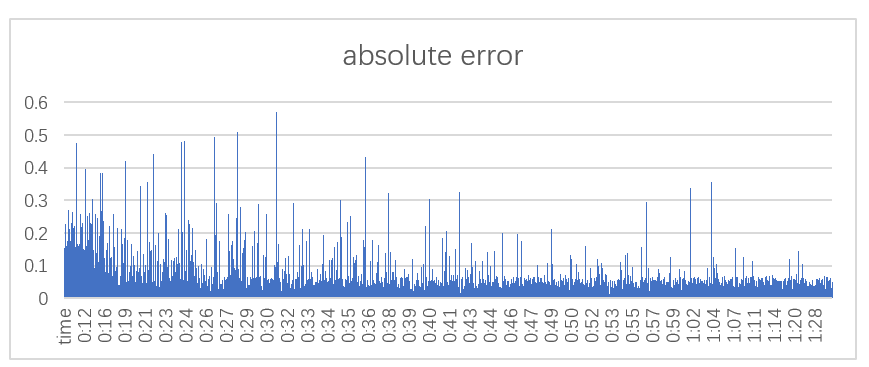
\includegraphics[width=1\columnwidth]{figure7.png}
\caption{Absolute error 2}
\label{fig:Absolute-error 2}
\end{figure}

In this paper, we use the method of statistical correlation analysis and the method of machine learning to determine the training factors. We have separately obtained the corresponding values of different factors and conducted a visual comparison study. The result is shown in the Fig.\ref{fig:Five-model-compare}.

\begin{figure}[tb]
\centering
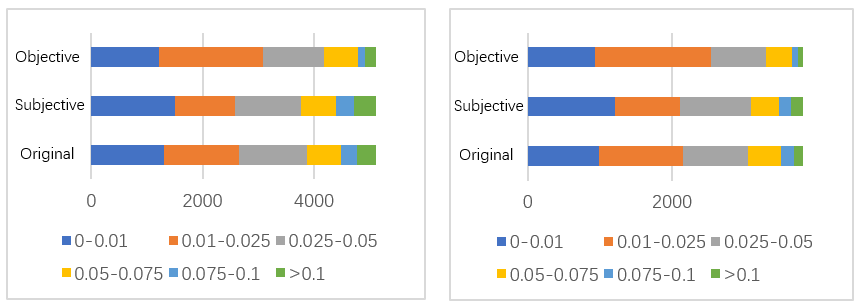
\includegraphics[width=1\columnwidth]{figure8.png}
\caption{Absolute error 3}
\label{fig:Absolute-error 3}
\end{figure}

However, we find that there are large errors in the calculation results in some cases (As shown in Fig.\ref{fig:Absolute-error 2} and Fig.\ref{fig:Absolute-error 3}). After discussion, we think there are mainly two possible causes of these errors, one is the impact of buses on data statistics and the other is the influence of the number of changeovers on the resistance of model accuracy. In order to calculate the attractiveness and radiation range of the business district more accurately, we divided the experimental samples and optimized the resistance value. And then we get the final model:

\begin{equation}
Attractive=\frac{Grade^{\alpha}*Mall^{\beta}*Area^{\gamma}*Reputation^{\delta}}{Time^{\mu}*\sqrt{Turn}}
\end{equation}

where $\sqrt{Turn}$ is resistance correction value through the transfer calculation. We use the optimization model for calculation, the results of the comparison shown in Fig.\ref{fig:Comparison-real-value}. 

\begin{figure}[tb]
\centering
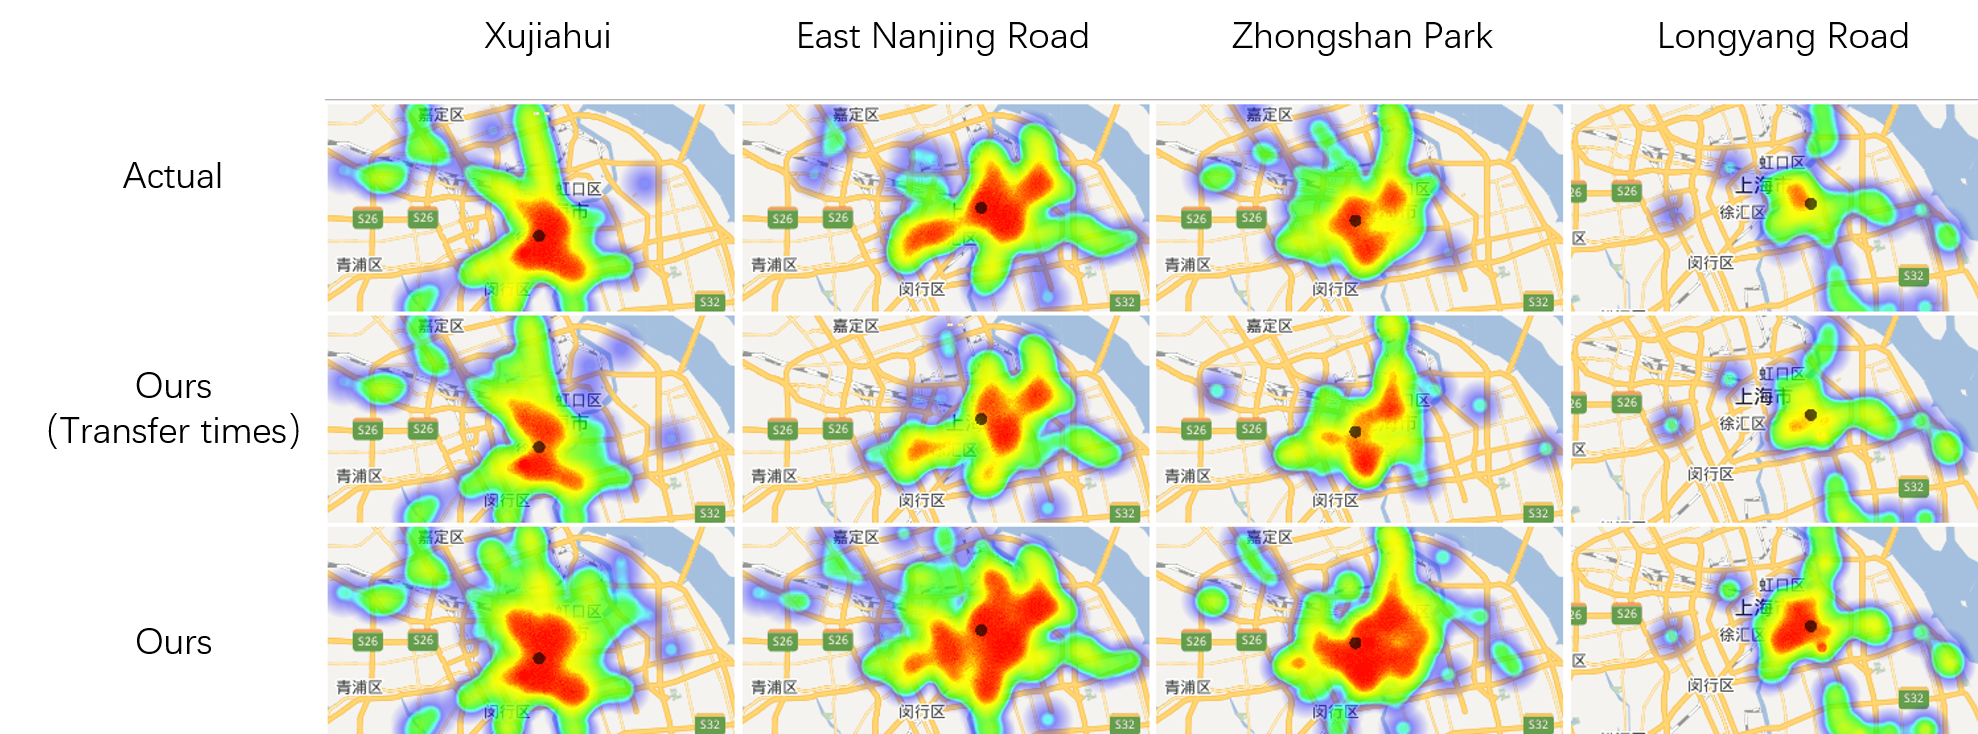
\includegraphics[width=1\columnwidth]{figure9.png}
\caption{Comparison of model and real value}
\label{fig:Comparison-real-value}
\end{figure}















\subsection{Deviation Analysis}

We use the original model to calculate, and then calculate the average error with the actual value, as shown in Fig.\ref{fig:Absolute-error 1}. Since the result of the calculation is a probability value between -1 and 1, we use the absolute error display.



We can find that in overall, the time cost and the positive or negative of error are no necessary connection. The reason for this result is that the underlying model does not apply to the current study, and after that we also perform an error study on the results of our model (formula 9), as shown in Fig.\ref{fig:Absolute-error 2}

It can be clearly seen in the diagram that the lower the time cost, the greater the error. At the same time, we compare the calculated values of Huff Model with different adjustment indices, as shown in the Fig.\ref{fig:Absolute-error 3}. Among this results, the error in the calculation is less than 0.025 that is much higher than that of the others, while the subjective index adjusted value can get more error than 0.01, which means that the application of objective index adjustment with better accuracy.

In a separate analysis of locations with larger errors, we found that the time cost for most of these sites to go to a business district was less than 10 minutes, which we believe is due to data error. We use the subway credit card data, but do not use the bus data which also occupy a large proportion of public transport. Customers near the business district prefer to take the bus to the nearest shopping district, which leads to errors in the actual probability values we measure. This error is mainly reflected in the over-estimation of the attraction of the nearest shopping district to residents, resulting in a larger error in subsequent calculations. However, we are temporarily unable to solve this problem in our work at this stage. In order to improve the model's applicability again and to optimize and improve it better, we removed the time-consuming sites less than 10 minutes and re-calculated the model. The results of the experiment are shown in the right of Fig.\ref{fig:Absolute-error 3}, of which there are 201 locations with 3819 groups data.

From the figure above, we can see that after we remove the locations with small time cost, the result has less error. Therefore, we think that the data errors are objective, but if we temporarily remove these locations with small time cost, the results will be more accurate.

By plotting the radiation profile with the actual values, we found a characteristic that was neglected in previous studies, which is the number of changeovers has a significant impact on the results. After analyzing the statistical results, we find it more attractive to go to the business district with fewer changeovers if the two business districts have similar resistance and attractiveness but obvious and different characteristics. We conducted an in-depth analysis of some of the locations and business districts with the above characteristics (business district: Zhongshan Park and Xujiahui, time cost: difference is less than 5min, which is considered consistent) as shown in Fig.\ref{fig:Transfer-times}. Zhongshan Park is the intersection of 2,3,4 lines and Xujiahui is the intersection of 1,9,11 lines.

Through visual analysis, we can clearly see that there is a connection between two locations with the same time cost. Among them, the purple spots are those who prefer Xujiahui, the green spots are those who prefer Zhongshan Park. As can be clearly seen from the figure, the closer geographical position does not mean to be more attractive, and the customer prefers to the business district with fewer changeovers with the same time cost. In other words, the more changeovers, the less attractive(more resistance) to customers. Hence, in our research, we need to consider the number of changeovers, whcih will improve the accuracy.





\begin{figure}[tb]
\centering
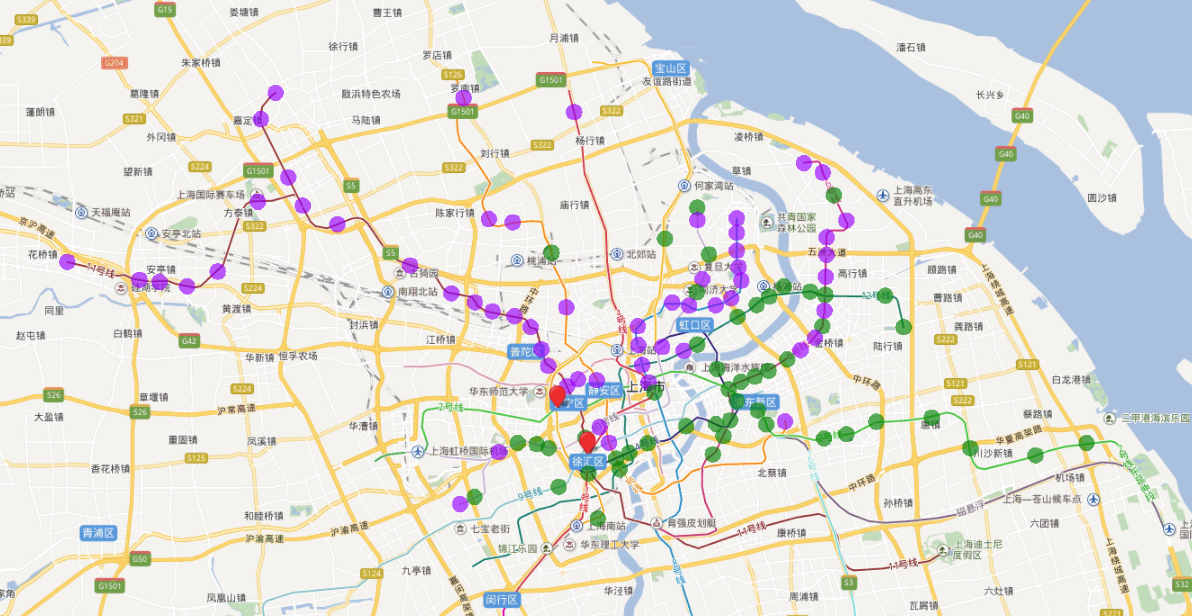
\includegraphics[width=1\columnwidth]{figure10.png}
\caption{Transfer times}
\label{fig:Transfer-times}
\end{figure}



\section{Case Study}

This section we use statistical analysis, user surveys and gray value calculation to verify our work.

\subsection{Model Comparison Study}

In this paper, we propose a customer-based method for radiation range division of business district, and the comparison about the division based on the business district as shown in Fig.\ref{fig:Real-range}.

Due to the data itself, in which the rail transit data are used only. Some errors are preduces when calculation based on the degree of attraction of the business district, which are mostly caused by the unattended flow of customers. Therefore, we think that when we divide the radiation range based on customers has greater advantages.

\begin{figure}[tb]
\centering
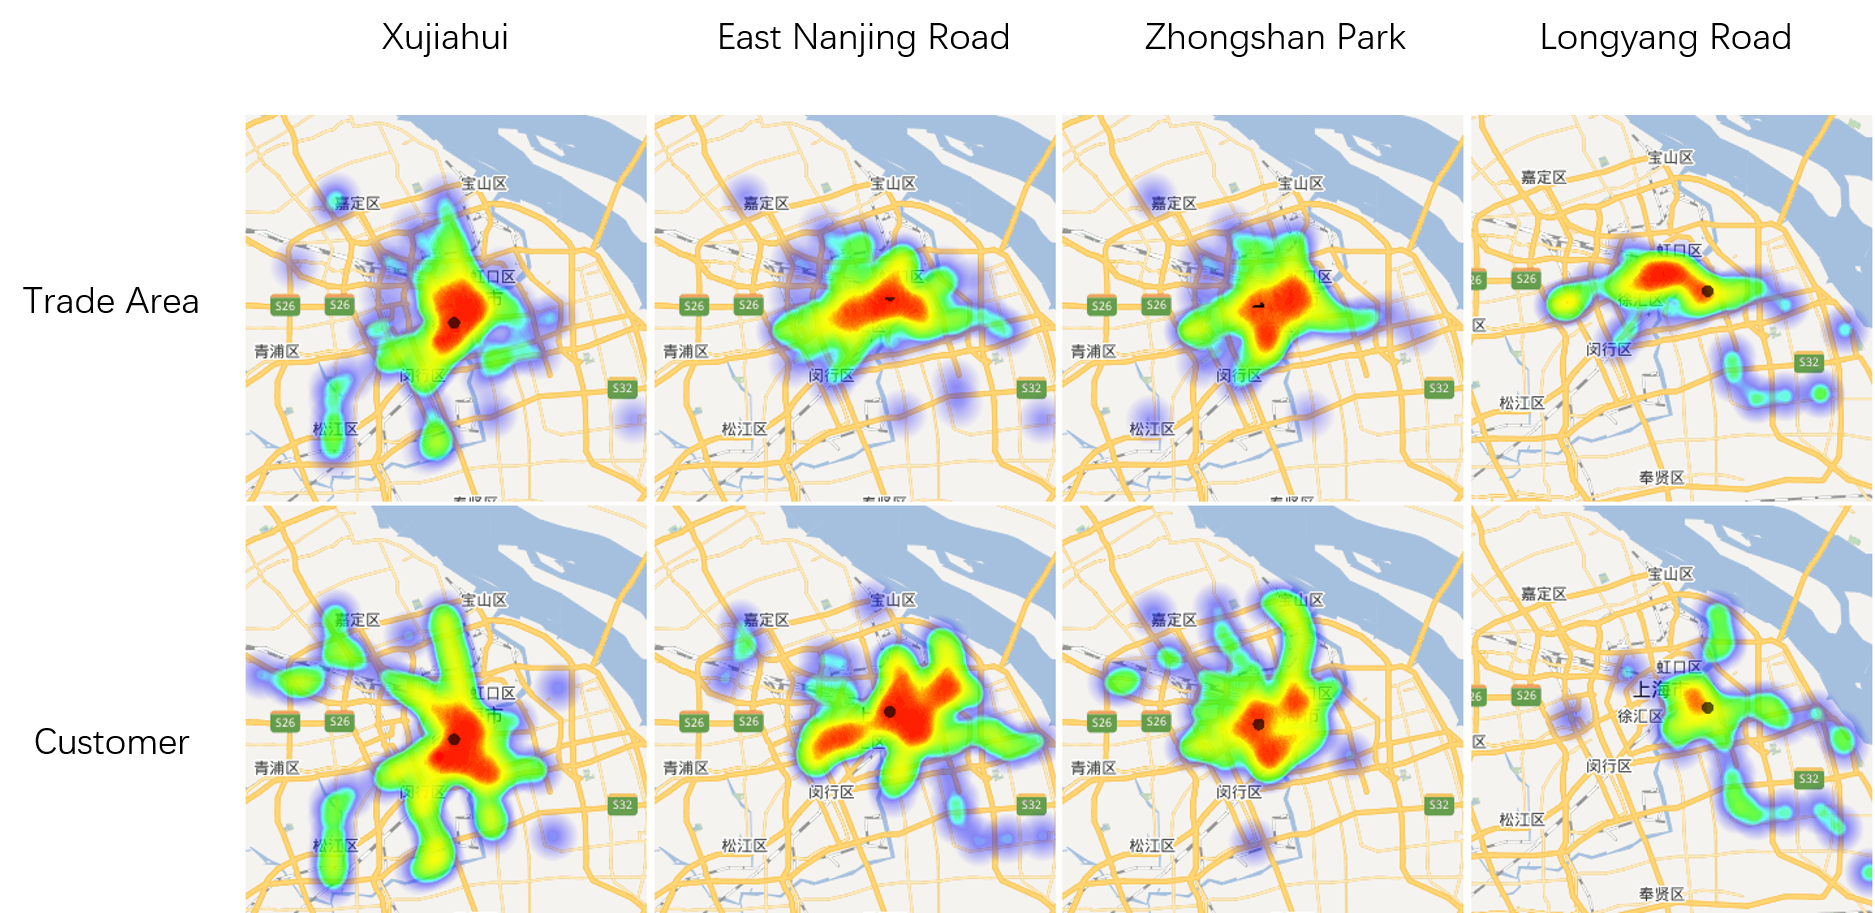
\includegraphics[width=1\columnwidth]{figure11.png}
\caption{Real range}
\label{fig:Real-range}
\end{figure}

We performed a model comparison, as shown in Fig.\ref{fig:Five-model-compare}, which shows the comparison between the Huff Model, the factors adjustment and our model. Since we found that the number of changeover lines has a great influence on the model calculation results, we further optimize the model. The comparison of calculation results is shown in Fig.\ref{fig:Real-range}.

\begin{figure}[tb]
\centering
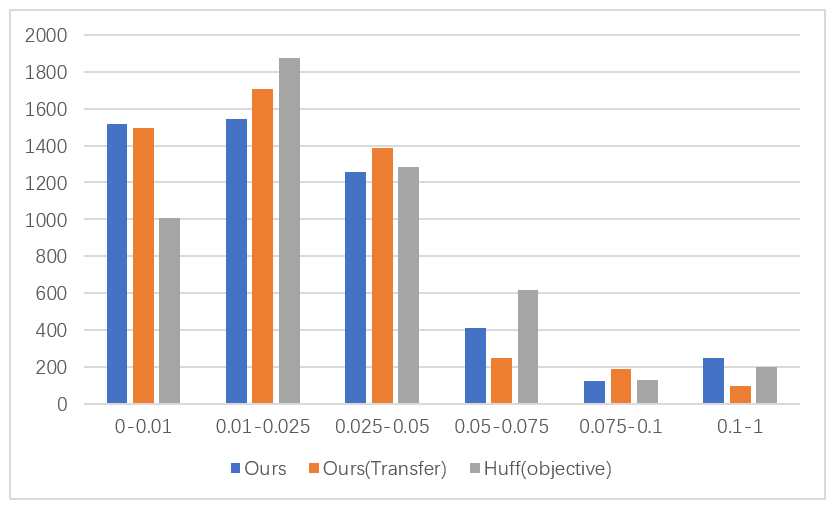
\includegraphics[width=1\columnwidth]{figure12.png}
\caption{Error comparison}
\label{fig:Error-comparison}
\end{figure}

We can clearly see that adding the number of line changes, the large expected attractiveness or the small expected resistance have been partially resolved. And the error calculated from the position is shown in Fig.\ref{fig:Error-comparison}. It can be seen in the figure that the error of our model is relatively smaller, and the accuracy after the adjustment of the number of changeover passes is more improved. It can be effectively explained that our model has more advantages than the rest of the models.

\subsection{Effectiveness Verification}





\section{Conclusions and Future Work}

In this paper, we propose a model that calculate the attraction from a business district to any place and a method of drawing the radiation range of the business districts in Shanghai. For the analysis and mining of one billion and six hundred million of RFID public transportation card data, we first conducted an analysis of crowds and settlements for verify whether our model is justified. Research on the attractiveness model of business district was then conducted. We conducted several error analysis and comparative analysis to optimize and verify our model, at the same time, we measure and draw the radiation range in the customer's perspective. Finally, we conducted a user study to see if their choices are consistent and compared these choices with our model and method. The results show that our research is relatively effective. However, we find that in some cases our work can not solve the problem well, which indicating that there are still some limitations in the research at this stage.

In the study of the attraction model of the shopping district, we found that in Shanghai, the number of changeovers has a great influence on the choice of business district. In this paper, only six variables were used to prevent overfitting, but experiments confirmed that this is enough to study the attractiveness and radiation range of the district. In addition, through the above research, we think the research in this paper can effectively forecast the urban business planning, and provide a good guide for the retail sales decision-makers.

This article constructs the attraction model of Shanghai's business district at this stage. With the rapid development of cities and commerce, many of the influencing factors used in the past may now lose their important position which requires us to pay attention to the details of the latest urban development in the study of business district. For example, the development of PTS replaced the traditional spatial distance to time cost, while the commercial area produced smaller differences due to commercial development. Hence, the attraction research of the business district will be based on economic and regional development which is constantly evolving. In addition, the model constructed in this paper is only applicable to large cities with convenient public transportation and commercial development. And in the future, we will conduct an in-depth study of small and medium-sized cities.

The research in this article is based on rail transit data only. However, as far as we know, in cities like Shanghai, buses traffic occupy one third of public transport, which can not be overlooked. Therefore, we will focus on this part in next work.


% \hfill mds
 
% \hfill August 26, 2015

% \subsection{Subsection Heading Here}
% Subsection text here.

% needed in second column of first page if using \IEEEpubid
%\IEEEpubidadjcol

% \subsubsection{Subsubsection Heading Here}
% Subsubsection text here.

% needed in second column of first page if using \IEEEpubid
%\IEEEpubidadjcol

% An example of a floating figure using the graphicx package.
% Note that \label must occur AFTER (or within) \caption.
% For figures, \caption should occur after the \includegraphics.
% Note that IEEEtran v1.7 and later has special internal code that
% is designed to preserve the operation of \label within \caption
% even when the captionsoff option is in effect. However, because
% of issues like this, it may be the safest practice to put all your
% \label just after \caption rather than within \caption{}.
%
% Reminder: the "draftcls" or "draftclsnofoot", not "draft", class
% option should be used if it is desired that the figures are to be
% displayed while in draft mode.
%
%\begin{figure}[!t]
%\centering
%\includegraphics[width=2.5in]{myfigure}
% where an .eps filename suffix will be assumed under latex, 
% and a .pdf suffix will be assumed for pdflatex; or what has been declared
% via \DeclareGraphicsExtensions.
%\caption{Simulation results for the network.}
%\label{fig_sim}
%\end{figure}

% Note that the IEEE typically puts floats only at the top, even when this
% results in a large percentage of a column being occupied by floats.


% An example of a double column floating figure using two subfigures.
% (The subfig.sty package must be loaded for this to work.)
% The subfigure \label commands are set within each subfloat command,
% and the \label for the overall figure must come after \caption.
% \hfil is used as a separator to get equal spacing.
% Watch out that the combined width of all the subfigures on a 
% line do not exceed the text width or a line break will occur.
%
%\begin{figure*}[!t]
%\centering
%\subfloat[Case I]{\includegraphics[width=2.5in]{box}%
%\label{fig_first_case}}
%\hfil
%\subfloat[Case II]{\includegraphics[width=2.5in]{box}%
%\label{fig_second_case}}
%\caption{Simulation results for the network.}
%\label{fig_sim}
%\end{figure*}
%
% Note that often IEEE papers with subfigures do not employ subfigure
% captions (using the optional argument to \subfloat[]), but instead will
% reference/describe all of them (a), (b), etc., within the main caption.
% Be aware that for subfig.sty to generate the (a), (b), etc., subfigure
% labels, the optional argument to \subfloat must be present. If a
% subcaption is not desired, just leave its contents blank,
% e.g., \subfloat[].


% An example of a floating table. Note that, for IEEE style tables, the
% \caption command should come BEFORE the table and, given that table
% captions serve much like titles, are usually capitalized except for words
% such as a, an, and, as, at, but, by, for, in, nor, of, on, or, the, to
% and up, which are usually not capitalized unless they are the first or
% last word of the caption. Table text will default to \footnotesize as
% the IEEE normally uses this smaller font for tables.
% The \label must come after \caption as always.
%
%\begin{table}[!t]
%% increase table row spacing, adjust to taste
%\renewcommand{\arraystretch}{1.3}
% if using array.sty, it might be a good idea to tweak the value of
% \extrarowheight as needed to properly center the text within the cells
%\caption{An Example of a Table}
%\label{table_example}
%\centering
%% Some packages, such as MDW tools, offer better commands for making tables
%% than the plain LaTeX2e tabular which is used here.
%\begin{tabular}{|c||c|}
%\hline
%One & Two\\
%\hline
%Three & Four\\
%\hline
%\end{tabular}
%\end{table}

% Note that the IEEE does not put floats in the very first column
% - or typically anywhere on the first page for that matter. Also,
% in-text middle ("here") positioning is typically not used, but it
% is allowed and encouraged for Computer Society conferences (but
% not Computer Society journals). Most IEEE journals/conferences use
% top floats exclusively. 
% Note that, LaTeX2e, unlike IEEE journals/conferences, places
% footnotes above bottom floats. This can be corrected via the
% \fnbelowfloat command of the stfloats package.

% if have a single appendix:
%\appendix[Proof of the Zonklar Equations]
% or
%\appendix  % for no appendix heading
% do not use \section anymore after \appendix, only \section*
% is possibly needed

% use appendices with more than one appendix
% then use \section to start each appendix
% you must declare a \section before using any
% \subsection or using \label (\appendices by itself
% starts a section numbered zero.)
%

% you can choose not to have a title for an appendix
% if you want by leaving the argument blank

% use section* for acknowledgment
% \section*{Acknowledgment}


% The authors would like to thank...


% Can use something like this to put references on a page
% by themselves when using endfloat and the captionsoff option.
\ifCLASSOPTIONcaptionsoff
  \newpage
\fi



% trigger a \newpage just before the given reference
% number - used to balance the columns on the last page
% adjust value as needed - may need to be readjusted if
% the document is modified later
%\IEEEtriggeratref{8}
% The "triggered" command can be changed if desired:
%\IEEEtriggercmd{\enlargethispage{-5in}}

% references section

% can use a bibliography generated by BibTeX as a .bbl file
% BibTeX documentation can be easily obtained at:
% http://mirror.ctan.org/biblio/bibtex/contrib/doc/
% The IEEEtran BibTeX style support page is at:
% http://www.michaelshell.org/tex/ieeetran/bibtex/
\bibliographystyle{IEEEtran}
% argument is your BibTeX string definitions and bibliography database(s)
\bibliography{business}
%
% <OR> manually copy in the resultant .bbl file
% set second argument of \begin to the number of references
% (used to reserve space for the reference number labels box)
% \begin{thebibliography}{1}

% \bibitem{IEEEhowto:kopka}
% H.~Kopka and P.~W. Daly, \emph{A Guide to \LaTeX}, 3rd~ed.\hskip 1em plus
%   0.5em minus 0.4em\relax Harlow, England: Addison-Wesley, 1999.

% \end{thebibliography}

% biography section
% 
% If you have an EPS/PDF photo (graphicx package needed) extra braces are
% needed around the contents of the optional argument to biography to prevent
% the LaTeX parser from getting confused when it sees the complicated
% \includegraphics command within an optional argument. (You could create
% your own custom macro containing the \includegraphics command to make things
% simpler here.)
%\begin{IEEEbiography}[{\includegraphics[width=1in,height=1.25in,clip,keepaspectratio]{mshell}}]{Michael Shell}
% or if you just want to reserve a space for a photo:

% \begin{IEEEbiography}{Michael Shell}
% Biography text here.
% \end{IEEEbiography}

% if you will not have a photo at all:
% \begin{IEEEbiographynophoto}{John Doe}
% Biography text here.
% \end{IEEEbiographynophoto}

% insert where needed to balance the two columns on the last page with
% biographies
%\newpage

% \begin{IEEEbiographynophoto}{Jane Doe}
% Biography text here.
% \end{IEEEbiographynophoto}

% You can push biographies down or up by placing
% a \vfill before or after them. The appropriate
% use of \vfill depends on what kind of text is
% on the last page and whether or not the columns
% are being equalized.

%\vfill

% Can be used to pull up biographies so that the bottom of the last one
% is flush with the other column.
%\enlargethispage{-5in}



% that's all folks
\end{document}


